\chapter{Feasibility}
The system requirements are listed below:
\begin{itemize}
    \item This system needs real time location of a user. The mobile phones have already a GPS sensor so this system needs to run on a mobile device.
    \item This system must provide interaction within users. So to provide intraction of multiple mobile devices this system needs a server side application.
    \item In process of development to provide version controlling Git must be used as VCS.
\end{itemize}

\section{Technic Feasibility}
As technical feasibility study, the software, hardware, communication, labor force, legal and economical needs for the project is defined on the following sections.
\subsection{Software Feasibility}

This project depends on web and mobile technologies.

\textbf{Mobile Side Development}
\newline
The tools and development environments used for mobile side development of the
project are mentioned below.
\newline
• Android \cite{android}: Android is a mobile operating system based on the Linux kernel. Its
source code is licensed under open source licenses and it is developing by Google
and Open Handset Alliance. The top layer of Android’s architecture is called
The Application Framework layer and it provides many higher-level services to
applications in the form of Java classes. Android was chosen over iOS \cite{iOS} because
of publishing problems, restrictions and lack of design guidelines that come with
iOS. Also Android has much more marketplace over iOS as shown in Figure \ref{fig:marketplace}. 

\begin{figure}[!htbp]
\centering
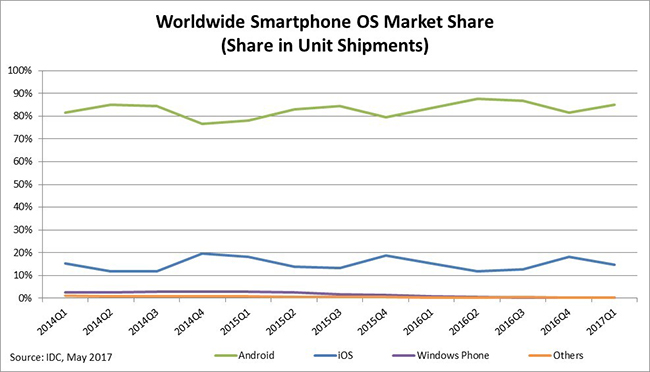
\includegraphics[width=\textwidth]{projectChapters/images/androidmarketplace.jpg}
\caption{Smartphone OS Market Share \cite{AndroidMarketShare}}
\label{fig:marketplace}
\end{figure}

• Android Studio: Android Studio is the official IDE for Android application
development, based on IntelliJ IDEA. Android Studio offers some advantages
over Eclipse, such as Gradle based flexible build system, advanced layout editor,
built-in Git source control and Maven library support \cite{androidStudio}.

• Android Sqlite Database: SQLite is a opensource SQL database that stores data to a text file on a device. Android comes in with built in SQLite database implementation. SQLite supports all the relational database features \cite{androidStudioSqlite}.

• Android Emulator: Android emulator lets prototype, develop and test Android applications without using a physical device \cite{androidEmulator}.

• Google Map API: Google Maps APIs give developers several ways of embedding Google Maps into web pages or retrieving data from Google Maps, and allow for either simple use or extensive customization \cite{googleMapAPI}.

• Operating System: An operating system in required for developing mobile application. Android Studio and Android Emulator can run on Windows, Linux or Mac OS \cite{mac}. We prefer to use Linux, because Linux needs relatively less resource and it's free to use. 

\textbf{Server Side Development}

The tools and development environments used for server side development of the
project are mentioned below.
\newline
• Java EE: Java EE is a collection of technologies and APIs for the Java platform designed to support "Enterprise" Applications which can generally be classed as large-scale, distributed, transactional and highly-available applications designed to support mission-critical business requirements. \cite{javaEETanim}
We have chosen JAVA EE platform because it is widely used by developers, its community is larger than most of its competitors, also it is a better option to use same language which is Java for the server side and mobile side development

• Eclipse: Eclipse platform which provides the foundation for the Eclipse IDE is composed of plug-ins and is designed to be extensible using additional plug-ins. Developed using Java, the Eclipse platform can be used to develop rich client applications, integrated development environments and other tools. \cite{eclipseTanim}
Eclipse can be used as an IDE for any programming language for which a plug-in is available. Eclipse has support for JAVA EE and Spring projects within its marketplace there are few IDEs that have these functionalities but Eclipse is open source and free.

• Sublime Text: Sublime Text is a proprietary cross-platform source code editor with a Python API. It natively supports many programming languages and markup languages, and functions can be added by users with plugins, typically community-built and maintained under free-software licenses. \cite{sublimeTanim}
Sublime Text is one of the greatest text editor in the world, almost every programming language is supported, we chosen it because of its Angular JS editing skills.

• MySQL : A database is a structured collection of data. It may be anything from a simple shopping list to a picture gallery or the vast amounts of information in a corporate network. \cite{mySQLTanim}
 MySQL is open-source and free. Developers didn't need to pay licence fee, also it gets updates regularly which makes it reliable.

• MySQL Workbench: MySQL Workbench is a unified visual tool for database architects, developers, and DBAs. MySQL Workbench provides data modelling, SQL development, and comprehensive administration tools for server configuration, user administration, backup and many more features. \cite{mySQLWorkTanim}
It is best option for MySQL development platform, when we compare to others such as Apache PhpMyAdmin it contains reverse and forward engineering tools, embedded UML diagram chart drawer tools, generating tables from models without complexity.

• Bootstrap: Bootstrap is a front-end development framework that enables developers and designers to quickly build fully responsive websites. The framework contains global CSS settings with built-in components and extensible classes in the form of typography, navigation, buttons and many other html elements. \cite{BootstrapTanim}
 We have chosen bootstrap because bootstrap equals platform in dependency, by developing on Bootstrap developers are able to run their code on every size of device such as phones,tables,computers,laptops and so on.

• Angular JS: AngularJS is a MVVM platform.  AngularJS is a structural framework for dynamic web applications. It lets you use HTML as your template language and lets you extend HTML’s syntax to express your application's components clearly and succinctly. AngularJS’s data binding and dependency injection eliminate much of the code you would otherwise have to write. \cite{AngularJSTanim}
 We have chosen Angular JS because it is officially supported and created by the Google. What that means is that it is more reliable than others. Also it has more libraries than other frameworks its community larger than others.

• Javascript : Javascript is a dynamic computer programming language. It is lightweight and most commonly used as a part of web pages, whose implementations allow client-side script to interact with the user and make dynamic pages. It is an interpreted programming language with object-oriented capabilities. \cite{JavascriptTanim}
 We have chosen it because it is almost only option for front end development. 

• Apache Tomcat : The Apache Tomcat software is an open source implementation of the Java Servlet, Java Server Pages, Java Expression Language and Java Web Socket technologies. The Java Servlet, Java Server Pages, Java Expression Language and Java WebSocket specification are developed under the Java Community Process. \cite{TomcatTanim}
 We have chosen Apache Tomcat because it is platform independent, we can run web server in a Linux machine. 

• Spring Framework :  The Spring Framework provides a comprehensive programming and configuration model for modern Java-based enterprise applications - on any kind of deployment platform.
\cite{SpringFrameTanim}
 A key element of Spring is infrastructural support at the application level: Spring focuses on the "plumbing" of enterprise applications so that teams can focus on application-level business logic,without unnecessary ties to deployment environments. Spring framework makes things easy for developers, such as creating Web Services, Controllers, web pages, database integrations, query implementations and so on. It is easy because most of the trivial processes are implemented by the framework, for example you don't need to open and close database connections by yourself when you execute a query in Java it is done by Spring it makes code less complex.

• STS: The Spring Tool Suite is an Eclipse-based development environment that is customized for developing Spring applications. It provides a ready-to-use environment to implement,debug,run,and deploy your Spring applications,including integrations for Pivotal tc Server, Pivotal Cloud Foundry, Git, Maven, AspectJ, and comes on top of the latest Eclipse releases. 
\cite{STSTanim}
We have chosen STS because it has embedded Eclipse plug-in integrated, there are other options such as Spring Incubator web page, but when you use others you have to implement some extra steps to import those projects in your local computer.

• Postman : API development tool that is a plug-in which comes as a packaged application in Chrome and is used to test the API services. Users can test the JSON REST based Web Services with this and make a API for cross device applications. 
\cite{PostmanTanim}
We have chosen Postman because its perfect GUI. You can save your REST calls and look it from other computers by registering. 

• Google Map API: Google Maps APIs give developers several ways of embedding Google Maps into web pages or retrieving data from Google Maps, and allow for either simple use or extensive customization \cite{googleMapAPI}. 
We have chosen Google Map API because it is free for the first 100.000 requests.

• PuTTy : PuTTy is a Telnet and SSH terminal software for Unix and Windows platforms that enables any users to remotely access computers over the Internet. 
\cite{PuttyTanim}
We have chosen PuTTy because it is platform independent and free.

• VNC : Virtual network computing (VNC) is a type of remote-control software that makes it possible to control another computer over a network connection. Keystrokes and mouse clicks are transmitted from one computer to another, allowing technical support staff to manage a desktop, server, or other networked device without being in the same physical location. 
\cite{VNCTanim}
We have chosen TightVNC as a tool for accessing remote server. TightVNC is also free and it is recommended by the community.

• WinSCP : This program is an open source free SFTP client, FTP client, Web DAV client and SCP client for Windows. Its main function is file transfer between a local and a remote computer.
\cite{WinSCPTanim}
 WinSCP is better option with its GUI for accessing remote file system. 
 
• JMeter : JMeter is an open source testing software. It is Java application for load and performance testing. JMeter is designed to cover categories of tests like load, functional, performance, regression, etc., and it requires JDK 5 or higher. \cite{JMeterTanim}
We have chosen JMeter to make HTTP calls in order to get server's client limit. It makes simultaneous calls between defined time periods and shows the summary of call outputs.

• htop : htop is an interactive system-monitor process-viewer and process-manager. It is designed as an alternative to the Unix program top. It shows a frequently updated list of the processes running on a computer, normally ordered by the amount of CPU usage. Unlike top, htop provides a full list of processes running, instead of the top resource-consuming processes. htop uses color and gives visual information about processor, swap and memory status.\cite{htopTanim}
We have chosen to monitor our server's stress test with htop because it has perfect GUI and it is really robust and easy to monitor.

\subsection{Hardware Feasibility}
The minimum hardware requirements for each program/IDE and
a system requirement compilation for development is shown in ~\ref{minreqmobile}, ~\ref{minreqserver}, ~\ref{androidhardware} based on the requirements.

\begin{table}[!ht]
\centering
\caption{Minimum System Requirement for Mobile Application Development}
\label{minreqmobile}
\begin{tabular}{|l|l|l|l|}
\hline
\textbf{Software}& \textbf{CPU (Ghz)} & \textbf{RAM (MB)}  & \textbf{Storage (GB)} \\ \hline
Linux OS \cite{linuxMinimumSystemRequirements} & \hfill 1 & \hfill 512 & \hfill 8 \\ \hline
Android Studio \cite{androidMinimumSystemRequirements} & \hfill 1.6 & \hfill 3072  & \hfill 8 (7 GB for SDK)\\ \hline
Android Emulator \cite{androidMinimumSystemRequirements} & \hfill unknown & \hfill 2048 & \hfill 1.5 \\ \hline
Minimum System Configuration & \hfill 1.6 & \hfill 5632 & \hfill 17.5 \\ \hline
\end{tabular}
\end{table}

\begin{table}[!ht]
\centering
\caption{Minimum System Requirement for Server Side Application Development}
\label{minreqserver}
\begin{tabular}{|l|l|l|l|}
\hline
\textbf{Software}& \textbf{CPU (Ghz)} & \textbf{RAM (MB)}  & \textbf{Storage (GB)} \\ \hline
Linux OS \cite{linuxMinimumSystemRequirements} & \hfill 1 & \hfill 512 & \hfill 8 \\ \hline
Eclipse \cite{eclipse} & \hfill 1.5 & \hfill 1024  & \hfill 1  \\ \hline
MySQL \cite{mysql} & \hfill 1 (2 core) & \hfill 2048 & \hfill 0.8 \\ \hline
MySQL Workbench\cite{mySQLWorkTanim} & \hfill 1 & \hfill 1024 & \hfill 0.2 \\ \hline
Apache Tomcat\cite{TomcatTanim} & \hfill 1 & \hfill 512 & \hfill 0.1 \\ \hline
JMeter\cite{JMeterTanim} & \hfill 1.2 & \hfill 512 & \hfill 0.2 \\ \hline
htop\cite{htopTanim} & \hfill 1 & \hfill 512 & \hfill 0.1 \\ \hline
Minimum System Configuration & \hfill 1.5 (2 core) & \hfill 8704 & \hfill 10.4 \\ \hline
Recommended System Configuration & \hfill 3 (4 core) & \hfill 16384 & \hfill 256 \\ \hline
\end{tabular}
\end{table}

\begin{table}[!ht]
\centering
\caption{Android Hardware Requirements}
\label{androidhardware}
\begin{tabular}{|l|l|l|l|}
\hline
            & \textbf{Minimum}    & \textbf{Recommended} \\\hline
CPU (Ghz) & \hfill 1      & \hfill 2     \\\hline
RAM (MB)      & \hfill 1024       & \hfill 1536        \\\hline
Storage (GB)   & \hfill 8     & \hfill 32       \\\hline
Version  & \hfill 5.0.0 (Lollipop)   & \hfill 7.1.1 (Nougat)      \\\hline
Sensors & GPS, Camera &  \\ \hline
Other & Internet Connection & \\ \hline
\end{tabular}
\end{table}

There is no restrictions for web clients. A web browser which supports WebGL and Internet connection is enough for using this system both for users and administrators.

\newpage
\subsection{Communication Feasibility}

Media files and path files are seperately stored on users android device. It so hard to send all of trip data one by one to one device to another without any loss. So we thought about that to compressing all files in a zip file before sending from mobile device to web server or vice versa. So we sended all data in one file. Also we will use less data bandwidth by compression. 

We had to compress photo files also. An uncompressed photo can be 5 MB but if we compress a photo using a compression technic the size of file will decreased seriously. Android provides three types of compression technic; WEBP, PNG and JPEG. We using JPEG for compression. Our decide three and performance comparison shown in Figure \ref{fig:photoCompression}.

\begin{figure}[!htbp]
\centering
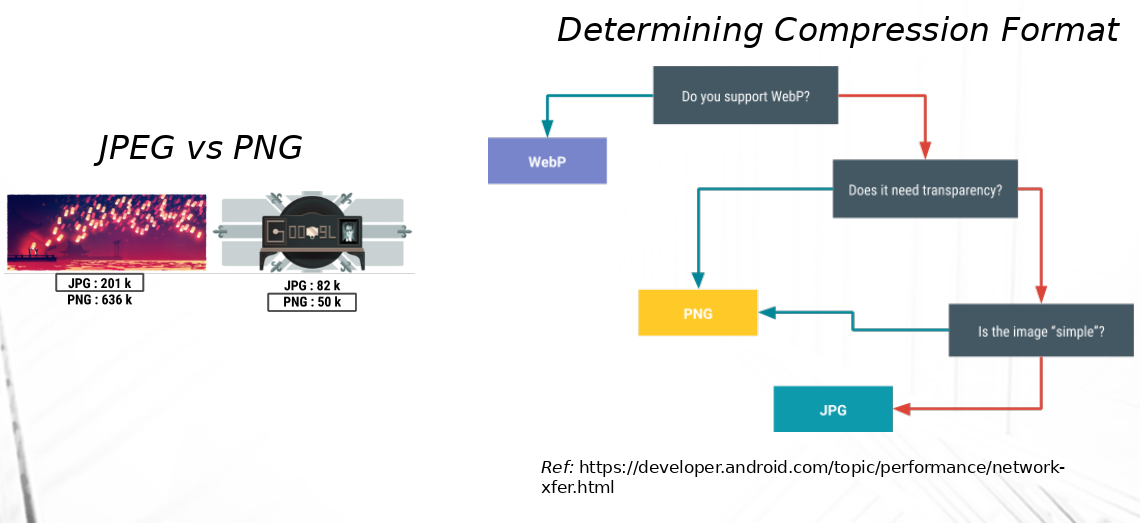
\includegraphics[height=38em]{projectChapters/images/photoCompression.png}
\caption{Photo Compression}
\label{fig:photoCompression}
\end{figure}

Our web server do not support WEBP format. PNG format is more successful over JPEG when there is poor color variety in a photo. If there is rich variety of colors JPEG is more successful over PNG format. We thought about that our application will used in real life and our photos has rich variety of colors. So we have chosen JPEG format to compress photos.

The Internet is the main communication technology used in this project. The
anticipated communication variables are shown in Table \ref{table:commparameters}.

\newpage
\begin{table}[!ht]
\centering
\caption{Communication parameters}
\label{table:commparameters}
\begin{tabular}{|l|l|r|r|}
\hline
\textbf{Description}                                                                   & \multicolumn{1}{l|}{\textbf{Symbol}} & \multicolumn{1}{l|}{\textbf{Values}} \\ \hline
Average Text File Size & A  & 50 kB \\ \hline
Average Video Size & B & 10 MB \\ \hline
Average Video Number Per User & C & 4 \\ \hline
Average Photo Size & D & 2 MB \\ \hline
Average Photo Number Per User & E & 20 \\ \hline
Average Sound Record Size & F & 1 MB \\ \hline
Average Sound Record Number Per User & G & 1 \\ \hline
Average Number Of Members in a Trip & H & 2 \\ \hline
Average Trip Data Size on Mobile(Unzipped) & I & 81 MB \\ \hline
Average Trip Data Size on Mobile(Zipped) & J & 56,7 MB \\ \hline
Average Trip Data Size on Web(Unzipped) & K & 162 MB \\ \hline
Average Trip Data Size on Web(Zipped) & L & 113 MB \\ \hline
Average Number of Upload Rate & M & 1000/month \\ \hline
Average Number of Download and View Rate & N & 7500/month \\ \hline
Average Size of Uploaded Trips & O & 55 GB \\ \hline
Average Size of Downloaded Trips  & P & 827 GB \\ \hline
Supposed Number of Users  & R & 10000 \\ \hline
Average Zip Compression Ratio \cite{zip} & S & 30\% \\ \hline
Server Data Rate Per Month & T & 827 GB \\ \hline
\end{tabular}
\end{table}


\[ I = G * F + E * D + C * B + A \]
\[ K = I * H \]
\[ J = I * (1 - S) \]
\[ L = K * (1 - S) \]
\[ O = J * M \]
\[ P = L * N \]
\[ T = MAX (O, P) \]

For this project we selected to rent a cloud computing system to make this project scalable. Scaleway \cite{scaleway} provides cloud computing services. Scaleway can provide multiple datacenters on different locations and developer tools on the machines. We selected scaleway for renting cloud server(s).

\begin{table}[!ht]
\centering
\caption{Scaleway package options \cite{scaleway}}
\label{scaleway}
\begin{tabular}{|l|r|r|r|r|}
\hline
\textbf{Specification}& \textbf{Starter} & \textbf{C2}  & \textbf{ARM64} & \textbf{C1} \\ \hline
CPU                             & 2x86 64bit & 8x86 64bit  & 8xARMv8 & 4xARMv7 \\ \hline
RAM                             & 2GB & 32GB & 8GB & 2GB \\ \hline
Storage                         & 50GB SSD & 50GB SSD & 200GB SSD & 50GB SSD \\ \hline
Number of public IPv4  & 1 & 1 & 1 & 1  \\ \hline
Bandwidth                       & 200Mbit/s & 800Mbit/s & 200Mbit/s & 200Mbit/s \\ \hline
Price                       & 2.99 Euro & 5.99 Euro & 9.99 Euro & 24.99 Euro \\ \hline
\end{tabular}
\end{table}

Based on the calculations above, the monthly data size will be around 827 GB. Scaleway provide 8 GB RAM and 200 GB storage with expandable options on ARM64 package shown on Table \ref{scaleway}. So we have to rent at least 5 ARM64 cloud servers from Scaleway.

\section{Labor Force Feasibility}
The resource chart for this project shown in ~\ref{fig:resource}.

\begin{figure}[!htbp]
\centering
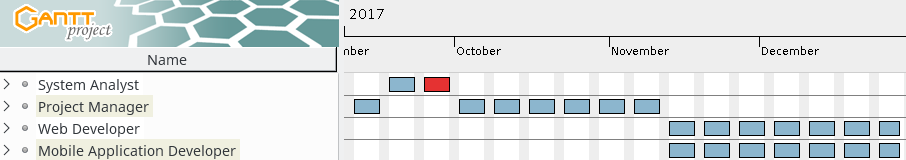
\includegraphics[width=\textwidth, height=10em]{projectChapters/images/resource.png}
\caption{Resource Chart}
\label{fig:resource}
\end{figure}

\section{Legitimate Feasibility}
Software which is used within the project does not face any legal issues. All of the
software used in the project contain license requirements. Users are responsible for
all shared content so any misusing of any sharing content is their risk. Sharing and publishing content is on their own risk, but if the users think that a profile, trip or comment has inappropriate content, they can create complaints about that. System administrators are in charge of assessing complaints. Admins can hide that specific content if they think it is inappropriate. Content that violates the user's personal rights will be blocked by this mechanism.

\newpage
\section{Time Feasibility}
Gannt diagram shown in Figure \ref{fig:ganttDeneme} and PERT diagram shown in figure ~\ref{fig:pertDiagram}.
\begin{figure}[!htbp]
\centering
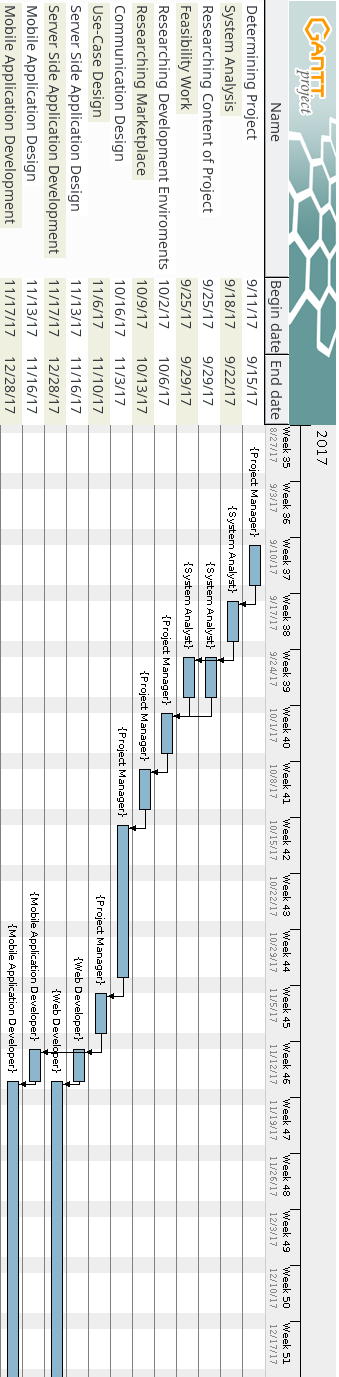
\includegraphics[scale= 0.64]{projectChapters/images/gant.png}
\caption{Gantt Diagram Drawing}
\label{fig:ganttDeneme}
\end{figure}

\begin{figure}[!htbp]
\centering
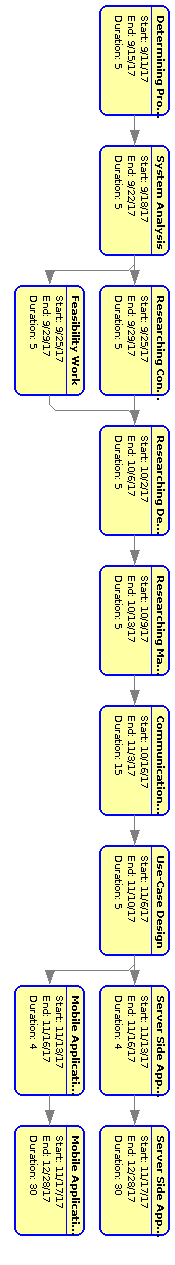
\includegraphics[scale = 0.7]{projectChapters/images/pert.png}
\caption{PERT Diagram Drawing}
\label{fig:pertDiagram}
\end{figure}

\newpage
\section{Economic Feasibility}
The salary determined by the government of the Republic of Turkey for engineers
is 3.500 TL \cite{muhendisMaas}. In a month there are 22 work days on average so an employee's daily salary is \ 3500 / 22 = 159,10\ TL. We thought that project manager must get a salary higher than other roles because project manager has more responsiblities than other roles. So we decided to give 6000 TL/month to project manager. In this sitiations project manager's daily salary is \ 6000 / 22 = 272,75\ TL.

\begin{table}[!h!]
\centering
\caption{Personnel cost table}
\label{tab:maas}
\begin{tabular}{|l|r|r|r|}
\hline
& \multicolumn{1}{l|}{\textbf{Time(Day)}} & \multicolumn{1}{l|}{\textbf{Price(TL/Day)}} & \multicolumn{1}{l|}{\textbf{Total(TL)}} \\ \hline
System Analyst   & 15                                      & 159,10                                      & 2.386,50                                 \\ \hline
Project Manager      & 35                                      & 272,75                                      & 9546,25                                 \\ \hline
Full Stack Developer     & 35                                      & 159,10                                      & 5.568,50                                 \\ \hline
Mobile Application Developer & 35                                       & 159,10                                      & 5.568,50                                  \\ \hline
General Total:      & \multicolumn{3}{r|}{23.069,75}                                                                                                  \\ \hline
\end{tabular}
\end{table}

The cost of computers used in the development process in 3.181 TL\cite{dell}. In the process 2 computer were used. A computer can be used for 2 years so 48 months in average lifetime. From here, we will find the cost of computer for 5 months is  \ (3.181*2)/(5/48) = 662\ TL. General Mobile GM6 used in the development process is 900,00 TL\cite{gm6}. It can be used for 12 months in average lifetime. From here we will find the cost of phone for 5 months as \ 900,00*(5/24) = 375\ TL. Mothly price of servers is \ 9.99 * 5 = 49,95\ Euro = 227,09 TL. We need this servers after 17 November 2017 due to 28 December 2017. For this 41 days servers price is \ 227,09 * (41 / 30) = 310,35\ TL. Considering these expenditures, the cost of hardware and software cost is 1.409,00 TL. The project development cost is \ 23.069,75 + 1.346,00 = 24.415,75\ TL.

\begin{table}[!h!]
\centering
\caption{Hardware and software used for development cost table}
\label{tab:hardsoftcost}
\begin{tabular}{|l|r|}
\hline
\textbf{Components}             & \multicolumn{1}{l|}{\textbf{Price (TL)}} \\ \hline
Eclipse \cite{eclipse} & 0,00 \\ \hline
Android Studio \cite{androidStudio} & 0,00 \\ \hline
2* Dell Vostro 5468 \cite{dell} & 662,00 \\ \hline
General Mobile GM6 \cite{gm6} & 375,00                            \\ \hline
2* Github Account                  & 0,00                            \\ \hline
Scaleway Server                  & 310,35                           \\ \hline
General Total:                  & 1.346,00                            \\ \hline
\end{tabular}
\end{table}

An administrator is absolutely necessary to run monitor and maintain the system. This administrator can get 3.500,00 TL/month salary and can use an average configurated computer. Toshiba Satellite L9W \cite{toshiba} is 1.000 TL and it is enough for administrator. We must provide an Internet connection for administrator. Türk Telekom provides an unlimited Internet package with 49,90 TL monthly \ref{ttnet}. Server cost has been calculated as 227,09 TL per month. So maintaining this system costs 1000 TL for administrator computer paid for once and \ 3.500,00 + 227,09 + 49,90 = 3.121,99\ TL per month.